\documentclass[12pt,addpoints, a4paper]{exam}
\usepackage[utf8]{inputenc}
\usepackage[table]{xcolor}
\usepackage{multicol}
\usepackage{graphicx}

%This block of commented code translates default words to Spanish
%-------------------------------------------------------------
%\pointpoints{punto}{puntos}
%\bonuspointpoints{punto extra}{puntos extra}

%\totalformat{Pregunta \thequestion: \totalpoints{} puntos}

%\chqword{Pregunta}
%\chpgword{Página}
%\chpword{Puntos}
%\chbpword{Puntos extra}
%\chsword{Puntos obtenidos}
%\chtword{Total}

%\boxedpoints

\renewcommand{\arraystretch}{2}
%-------------------------------------------------------------

\begin{document}
%This code creates the text before the first question
%-------------------------------------------------------------------
\makebox[\textwidth]{Nom Prénom:\hrulefill}
%\vspace{5mm}
\begin{center}
\fbox{\fbox{\parbox{5.5in}{\centering
\LARGE \textbf{Devoir Surveillé : Addition et Soustraction de nombres relatifs}}}}
\end{center}





\qformat{\large \textbf{Exercice \thequestion} \dotfill \thepoints}
%-------------------------------------------------------------------

%Here, the questions begin
\begin{questions}
\vspace*{0.7cm}
%First question below

\question 

\begin{parts}
\part Compléter le tableau en indiquant par "+" ou "-" le signe de chaque somme

%\vspace{\stretch{1}} %Equally distributes the available space
\hspace*{-1.7cm}
\begin{tabular}{|c|c|c|c|c|c|}	
	\hline
	\cellcolor{gray}\textbf{Somme} &    $353 + (-554,8)$ &  $13,5 + (-11,5)$ & $ -56,9 + (+59,6)$ & $ 44,7 + (-78)$ & $ -82 + (-223) $ \\
	\hline
	\cellcolor{gray}\textbf{Signe} & & & & & \\
	\hline	
\end{tabular}



\part  Compléter le tableau suivant avec le résultat des opérations correspondantes.

%\hspace*{-1cm}
\begin{tabular}{|c|c|c|c|c|c|c|}	
	\hline
	\rowcolor{gray} ~~\textbf{a}~~ &    ~~\textbf{b}~~ &  ~~\textbf{c}~~ & ~~~~~~\textbf{$a+b$}~~~~~~ & ~~~~~~\textbf{$(a+b)+c$}~~~~~~ & ~~~~~~\textbf{$(a+b)-c$}~~~~~~ \\
	\hline
	$+5$ & $-4$ & $-2$ & & & \\
	\hline	
	$-6,2$ & $-5,1$ & $4,9$ & & & \\
	\hline
	$+3,7$ & $0$ & $4,3$ & & &  \\
	\hline
	$-${\Large $\frac{35}{3}$} & +{\Large $\frac{41}{3}$} & -{\Large $\frac{49}{3}$} & & &  \\
	\hline	
\end{tabular}


\end{parts}

%\droptotalpoints %Prints the number of points in this question

\vspace*{0.5cm}
%----------------------------------------------------------------------------
%----------------------------------------------------------------------------
%----------------------------------------------------------------------------
\question
Problèmes (Détailler les calculs effectués):

\begin{parts}
	\part Combien de temps a vécu le mathématicien Pythagore (né en 580 av JC; mort en 497 av JC) ?
	
	\part Sur Mars, la température minimale est de $-140$ºC, et l'amplitude thermique (écart entre la température minimale et la maximale) est de $170$ºC : calculer la température maximale sur Mars.
	%\vspace{0.1cm}
	\part Du haut d'un viaduc, Xavier s'élance dans le vide, les pieds attachés à un élastique.
	Il descend de 25 m, remonte de 12 m, redescend de 8 m, remonte de 3 m, redescend de 1 m et remonte de 0,5 m, il s'arrête là.
	Calculer (en une seule expression) à combien de mètres sous le viaduc Xavier s'est immobilisé.
\end{parts}

%\vspace*{0.5cm}
\clearpage
%----------------------------------------------------------------------------
%----------------------------------------------------------------------------
%----------------------------------------------------------------------------
\question

\begin{parts}
\part Placer les points $A(-2;4)$, $B(-1;-3)$, $C(2;3)$, $D(1;-4)$ et $E(0;4)$ sur le repère orthogonal fourni.
\part Citer deux points d'ordonnées opposées.
%\part Quelle est la nature du quadrilatère $BDCE$ ? (Justifier) 
\part Placer le point $F$ en ajoutant -2 à l'abscisse de $C$ et en soustrayant 3 à son ordonnée. %\par
Donner ses coordonnées.	
\end{parts}	

\vspace*{0.5cm}	
%----------------------------------------------------------------------------
%----------------------------------------------------------------------------
%----------------------------------------------------------------------------
\question
Simplifier les expressions algébriques suivantes, puis les calculer
\begin{parts}
\part $A = (-100) + (-57) + (+12) + (+102) + (+56) + (-12)$
\part $B = (-4,4) + (+4) + (-3,1) + (-1,5) + (+0,4) + 0,5$
%\part $C = (-6,2) + (-5,7) + (-4,8) + (+5,6) + (+4,7) + 6,1$
\part $C = (+2) - (-3) + (-5) + (+4) - (+2) + (-4)$
%\part $D = (-16,7) - (-3,2) + (+4,8) - (+3,3) + (+2,5) - (-5,5)$
\end{parts}	


\question Choisir la (ou les) bonne(s) réponse(s) parmi celles proposées. 
%
\begin{multicols}{2}


\begin{parts}
\part
On peut dire que deux nombres sont opposés lorsque ...
\begin{checkboxes}
	\choice Leur somme est égale à 0
	\choice Leur somme est égale à 1
	\choice Leur différence est égale à 0	
\end{checkboxes}	


\part
Rangée dans l'ordre croissant, la liste \{$-8; -9,4; -7; 6; -7,6$\} devient ...
\begin{checkboxes}
	\choice \{$6; -7; -7,6; -8; -9,4$\} 
	\choice \{$-9,4; -8; -7; -7,6; 6$\}
	\choice \{$-9,4; -8; -7,6; -7; 6$\}
\end{checkboxes}	
\vspace*{0.5cm}
\part
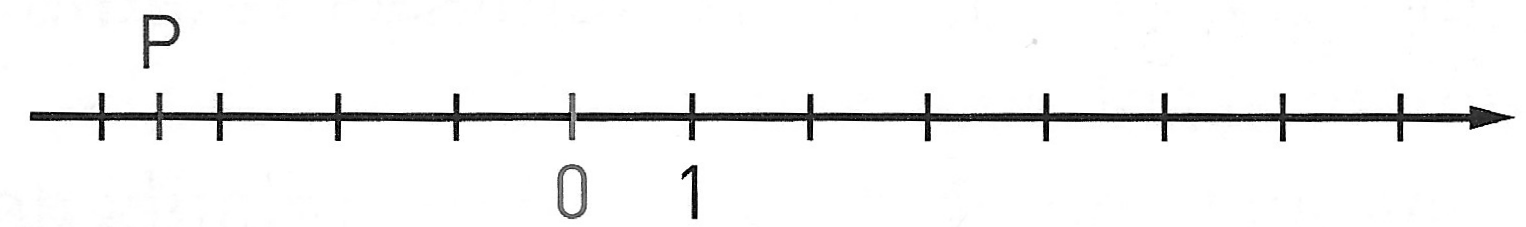
\includegraphics[scale=0.15]{./img/axe3}\\
En observant cet axe gradué, on peut dire que l'abscisse de P est ...

\begin{checkboxes}
	\choice entre $-4$ et $-3$
	\choice entre $3$ et $4$
	\choice inférieure à $-3$
\end{checkboxes}

\part
$(-12) + (+7) - ... = 3$\\
Le nombre manquant dans cette opération est 
\begin{checkboxes}
	\choice $2$
	\choice $+8$
	\choice $-8$
\end{checkboxes}
\end{parts}	
\end{multicols}
%-------------------------------------------------------------------

\clearpage
\makebox[\textwidth]{Nom Prénom:\hrulefill}
\vspace*{1cm}
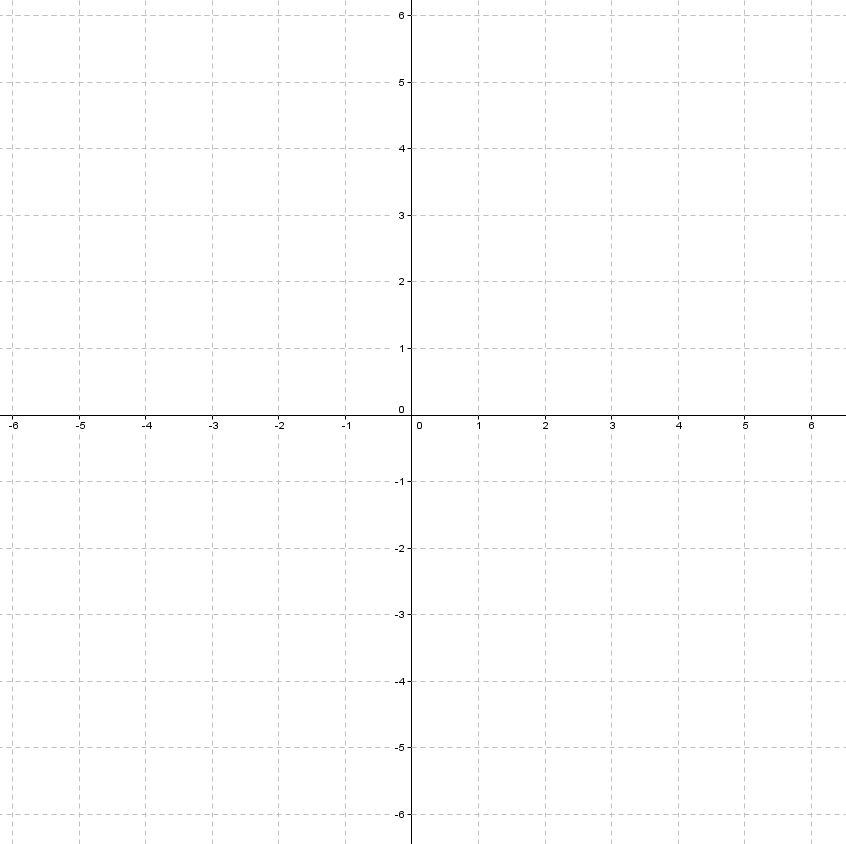
\includegraphics[scale=1]{./img/repere}

\end{questions}

%\clearpage
%\begin{center}
%\combinedgradetable[h][questions]
%\end{center}

\end{document}

%The next two questions are multiple choice examples
%-------------------------------------------------------------------
%\question Which of these guys invented time
%
%\begin{oneparchoices}
% \choice Stephen Hawking 
% \choice Albert Einstein
% \choice Isaac Newton
% \choice This makes no sense
%\end{oneparchoices}
%
%\question Which of these guys published a paper on Browninan Motion
%
%\begin{checkboxes}
% \choice Stephen Hawking 
% \choice Albert Einstein
% \choice Isaac Newton
% \choice I don't know
%\end{checkboxes}